\documentclass{article}

\usepackage{amsmath}
\usepackage[utf8]{inputenc}
\usepackage{graphicx}
\usepackage{tikz}

% Cite authors. Use \citeauhor*{auth}
\usepackage[numbers]{natbib}
\bibliographystyle{plainnat}

\title{Theoretical Grounds and Market Adaptations of Financial Fx Options \\ \large A summary in plain english and some math}

\author{Gerardo Dur\'an Mart\'in}

% Allows to define variables in math Formula setting them to the left
\renewcommand*\descriptionlabel[1]{\hspace\leftmargin$#1$}

% Cite as: AUTHOR(YEAR) style
\newcommand{\Mycite}[1]{%
 \citeauthor{#1}(\citeyear{#1})}


\begin{document}
\graphicspath{ {images/} }
\maketitle

\section{The Context}

In its simplest form, a European call (put) option gives the buyer the right, albeit not the obligation, to buy (sell) some underlying asset at a specified future period at a set price called the strike price.\\

Options can trade either Over The Counter or at exchanges such as the Chicago Board Options Exchange or the International Securities Exchange in the U.S.\cite{sec_listed} and Mexder in Mexico \citep{mexder}.\\

According to the Bank of International Settlements, the Daily Average Turnover Value (DATV) for exchange traded options was 1,278,571 USD in 2015. Although the current DATV for is not as big as it was at its peak in august 2007, the option markets are still relevant for today's financial needs.

\begin{figure}[h!]
    \centering
    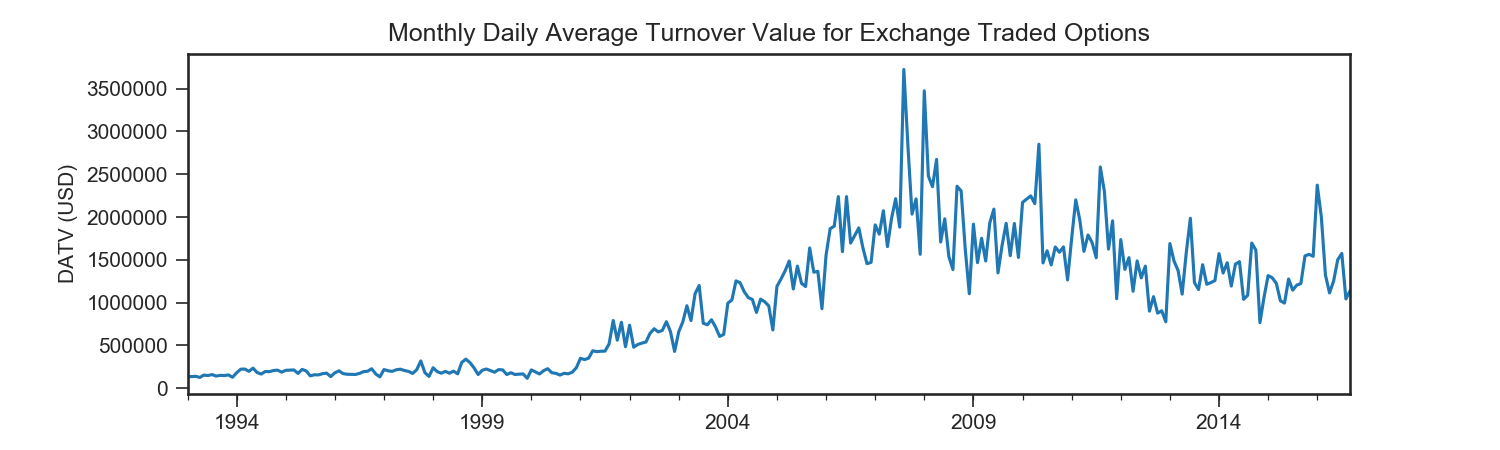
\includegraphics[width=1.0\textwidth]{DAVT}
    \caption{DAVT from 1993 to 2016}
\end{figure}

Popular as they are, pricing the simplest of them all, sometimes known as \textit{plain vanilla options}, bear within a vast mathematical background that relies on assumptions about the markets in which the options are trading and the behavior of the underlying assets from which their price is derived.\\

Understanding the groundwork required to price these options bring about a better understanding of the strengths and weaknesses of the model. Herein is a brief summary for the work to be written as a thesis.

\section{Theoretical Grounds}
The pricing theory of options had its first mayor breakthrough after Robert Black and Myron Scholes published a paper in which they derived a formula for a European option theoretical price. As pointed out by \Mycite{pre_bs},

\begin{quote}
``The breakthrough of \Mycite{black_scholes}, was to realize that the expected return of the option price should be the risk free rate and that by holding a certain amount of stock, now referred to as the delta, the option position could be dynamically completely hedged.''
\end{quote} 

The Black Scholes Model developed in 1973 relates to the pricing of options whose underlying is a stock. Said stock is assumed to follow a geometric Brownian motion. This is, given a stock $S_t$, its change can be represented as the following stochastic differential equation.

\begin{equation}
    dS_t = r dt + \sigma dW_t 
\end{equation}

Where $r$ is the risk-free interest rate, $\sigma$ is the volatility, and $dW_t$ represents the infinitesimal change of a Brownian Motion movement.\\

In their paper, \Mycite{black_scholes}, introduce a way to hedge the position of an option by holding a certain amount of stocks and investing money at a risk free rate. Simply put, let $X(t)$ be a collection of assets known as a portfolio holding $a$ units of the underlying stock and $\$b$ invested at the risk-free rate $r$, some value for an option depend on the stock $C(t)$, they derived a formula that explains the movements in the value of the option $C(t)$ in terms of the movements in value for the portfolio $X(t)$ i.e.

\begin{equation}
    dX(t) = dC(t)
\end{equation}

The solution to this last equation yields the Black-Scholes-Merton Partial Differential Equation.

\begin{equation}
    \frac{\partial C}{\partial t} + \frac{1}{2}\sigma^2 S^2 \frac{\partial^2 C}{\partial S^2} + rS\frac{\partial C}{\partial S} - rC = 0  
\end{equation}\\


Solving the Black Scholes PDE yields the analytical formula for pricing a European call option

\begin{equation}
    C(S_t,  K, \sigma, r, \tau) = S_t \Phi(d_+) - Ke^{-r\tau}\Phi(d_-)
\end{equation}

where
\begin{description}
	\item[d_{\pm} = \frac{1}{\sigma\sqrt{\tau}}\left(\log\frac{S_t}{K} \pm (r - \frac{\sigma^2}{2})\tau\right)]
    \item[\tau] is the time to maturity in years
    \item[\sigma] is the volatility of the stock
    \item[S_t] is the price of the stock at time $t$
    \item[K] is the strike price
\end{description}

\section{Market Adaptations}
Although the \citeauthor{black_scholes} model is mathematically consistent, it fails to take account some factors that affect markets today. Said factors must be corrected in order to correctly price the value of options. Two of those factors are the \textit{volatility smile} and the assumption of the existence of a \textit{risk-free rate}.

\subsection{Volatility Smile}
Denote $\sigma_K$ the volatility for an option that matures in $\tau$ years and has a strike of $K$. \\

According to the BSM model, $\sigma_i = \sigma_j$ for every $i$, $j$. In reality, markets observe different values of volatility at different levels of strikes. Furthermore, not all values of the volatility smile are know at each strike, so a method of interpolation is necessary to solve this problem.

\begin{figure}[h]
    \centering
    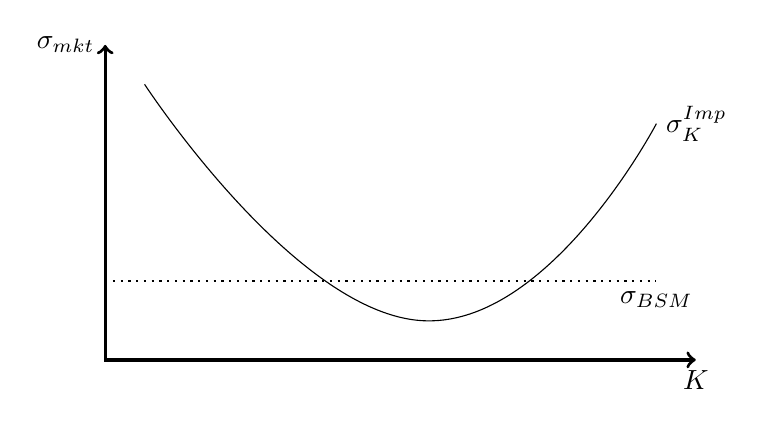
\begin{tikzpicture}
        \draw [very thick, <->] (0,4) node[left]{$\sigma_{mkt}$} to (0,0) to (7.5,0) node[below]{$K$};
        \draw plot[smooth, tension = .9] coordinates{ (0.5,3.5) (4,0.5) (7,3)};
        \node [right] at (7,3) {$\sigma^{Imp}_K$};
        \draw [dotted, thick] (0,1) to (7,1) node [below] {$\sigma_{BSM}$};
    \end{tikzpicture}
    \caption{Representation of the volatility smile}
\end{figure}

Another problem emerges in Fx markets, where the implied volatility is quoted in terms of the \textit{moneyness} of the option i.e. its Delta \citep{wys}, and it poses a new problem to go from Delta to the corresponding associated strike for the same volatility.

\subsection{Curve Construction and Selection}
Assuming there exists a risk free rate, this can be known at various tenors from a zero coupon bond trading in the market, a problem then arises once we try to price an option at a maturity not defined for the tenors trading in the market. To solve this, we can fit a curve for the known tenors such that are market-consistent and imply no arbitrage. \\

\begin{figure}[h]
    \centering
    \begin{tikzpicture}[x=70, y=50]
        \draw [very thick, <->] (0,2) node[left]{$r$} to (0,0) to (3.5,0);
        \draw plot[smooth, tension = .9] coordinates{ (0.6,0.5) (1.1,0.9) (3,1.5)};
        \fill (0.6, 0.5) circle[radius=2pt];
        \fill (1.1, 0.9) circle[radius=2pt];
        \fill (3, 1.5) circle[radius=2pt];
    \end{tikzpicture}
    \caption{Curve Interpolation of a ZCB with Known Tenors}
\end{figure}

Under current market conditions, the existence of a risk free rate is a fallacy. Ever since the aftermath of the credit crisis of 2007, markets have assumed a multicurve paradigm \citep{len}. No longer are the rates at which one estimates future cash flows are the same as those as used for discounting.

\section{Thesis Statement}
As pointed out above, the valuation of an option requires mathematical background in stochastic processes, numerical methods and partial equations in order to price an option under a risk-neutral, free-arbitrage market.\\

The aim of this work is to develop the mathematical theory under which financial options are priced. We will then question the effectiveness of the model and how can it be adapted to real market constraints. Concretely, we will focus on the calibration of two parameters of the model: its volatility and the \textit{risk-free} interest rate.

\newpage
\nocite{*}
\bibliography{ref}
\end{document}